%!TeX program = xelatex
\documentclass[12pt,hyperref,a4paper,UTF8]{ctexart}
\usepackage{SJTUReport}
\ctexset{bibname = References}


%%-------------------------------正文开始---------------------------%%
\begin{document}

%%-----------------------封面--------------------%%
\cover

%%------------------摘要-------------%%
\newpage
\begin{abstract}
    This report investigates the evolution of decision-making research, tracing its development from philosophical foundations to contemporary interdisciplinary approaches that integrate psychology, neuroscience and mathematics. We emphasize perceptual decision-making, particularly through experiments utilizing visual stimuli in monkeys, which illuminate the neural mechanisms underlying decision processes. The Competition Population Model is introduced to elucidate the interactions among neuronal populations and their inhibitory dynamics. Additionally, we examine alternative decision-making frameworks, including the drift-diffusion model, to provide a comprehensive understanding of the decision-making landscape. The report further explores the intricate relationship between human decisions, determinism, and free will, referencing the Libet experiment to illustrate the unconscious processes that precede conscious decision-making. Ultimately, this work underscores the complex neural foundations of decision-making and contributes to the ongoing discourse regarding the nature of choice and volition.
\end{abstract}

\thispagestyle{empty} % 首页不显示页码

%%--------------------------目录页------------------------%%
\newpage
\tableofcontents

%%------------------------正文页从这里开始-------------------%
\newpage
\section{Introduction}
The study of decision-making has a rich history that extends back to early philosophical inquiries into human behavior and rationality. In ancient times, philosophers pondered the nature of choice and the factors influencing human actions. These early reflections laid the groundwork for a more systematic understanding of decision-making, yet they lacked a formalized framework. It was not until the late 19th century that scholars began to explore decision-making through a more empirical lens, focusing on psychological and behavioral aspects rather than strictly mathematical models.

As the 20th century progressed, the integration of mathematics into decision-making research became more pronounced. The development of Expected Utility Theory by John von Neumann and Oskar Morgenstern in 1944 marked a significant turning point, providing a mathematical framework for understanding rational decision-making under uncertainty. This theoretical approach was further expanded by economists and psychologists who sought to quantify preferences and risks, paving the way for a more rigorous analysis of choices in various contexts.

In the late 20th and early 21st centuries, the study of decision-making evolved to incorporate insights from neuroscience and behavioral economics. Researchers began to examine the biological underpinnings of decision-making, exploring how brain structures influence choices and risk assessment. This interdisciplinary approach, often referred to as neuroeconomics, combined elements of psychology, biology, and mathematics, leading to a more comprehensive understanding of the decision-making process.

This report will focus on decision-making models developed around the year 2000 and beyond, highlighting key contributions and advancements in the field. In Section 2, we will discuss experiments conducted since the 1990s that have enhanced our understanding of perceptual decision-making. Section 3 will introduce one of the most widely used decision models, the Competition Population Model, and Section 4 will analyze the dynamics of this model in detail. In Section 5, we will explore alternative models introduced during the same period. Finally, Section 6 will examine recent research on more complex decision making processes that incorporate the concept of free will, a topic that remains an unresolved mystery.
%%------------------------正文页从这里开始-------------------%

\newpage

\section{Perceptual decision making}

In what follows, we focus on an experimental paradigm with visual random dot motion stimuli used for the study of perceptual decision making in monkeys (\cite{Salzman 1990} Salzman 1990; \cite{Roitman and Shadlen 2002} Roitman and Shadlen 2002; \cite{Gold and Shadlen 2007} Gold and Shadlen 2007). The stimulus consists of a random pattern of moving dots, where most, but not necessarily all, of the dots move coherently in the same direction Typically, two different directions of motion are used, for example upward or downward. The monkey has been trained to indicate the perceived motion direction by saccadic eye movements to one of two targets (\autoref{monkey1}).

\begin{figure}[h]
    \begin{center}
    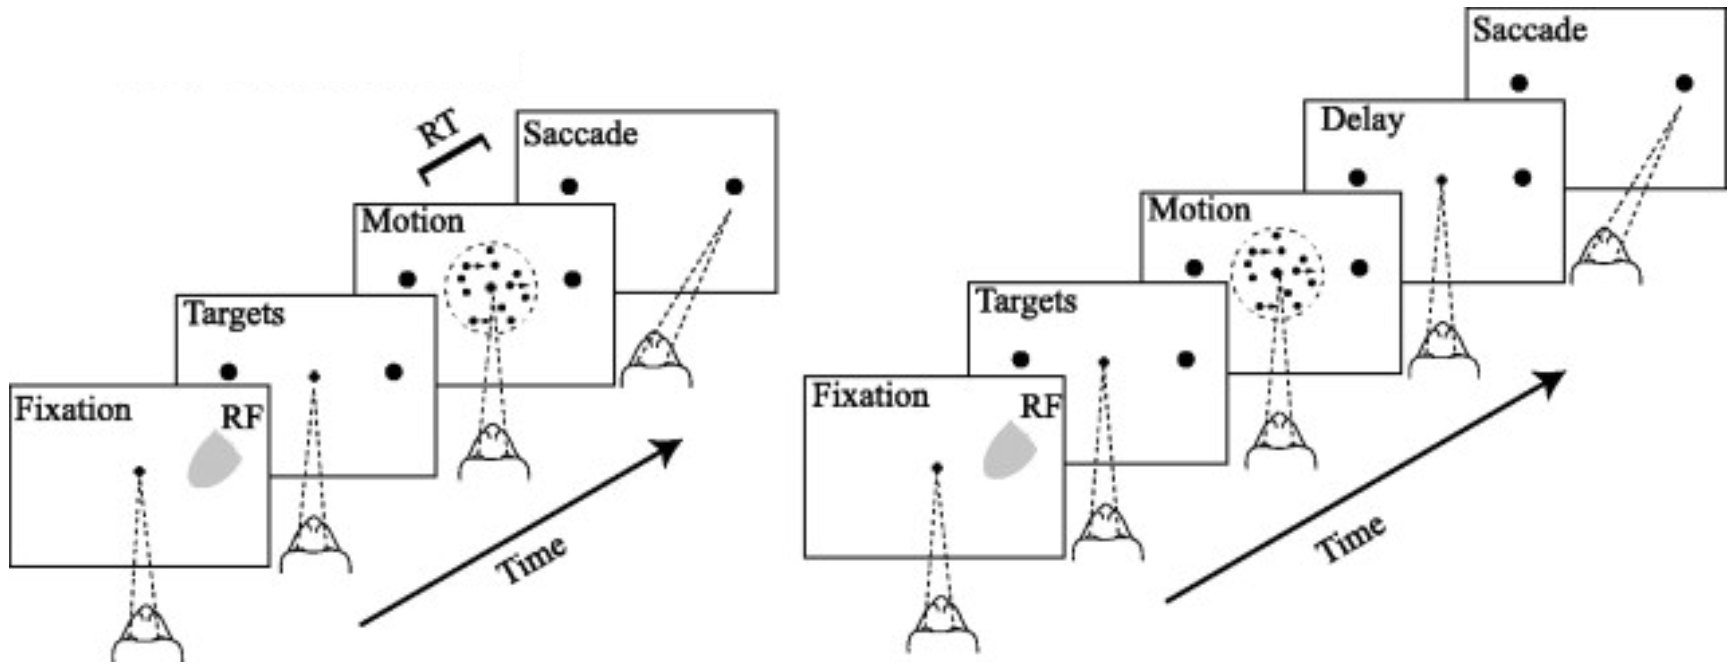
\includegraphics[width=0.9\textwidth]{monkey1.png}
    \caption{Perceptual decision making in monkeys.}
    \label{monkey1}
    \end{center}
\end{figure}

\subsection{Perception of motion}

Neurons in the middle temporal visual area (MT, also called V5) are activated by largescale motion stimuli. The receptive field of an MT neuron, i.e., the region of visual space that is sensitive to motion stimuli, is considerably larger than that of a neuron in the primary visual cortex. Different neurons in MT respond to different directions of motion, but just as in other parts of the visual cortex, area MT has a columnar structure so that clusters of neighboring neurons share receptive fields with a similar preferred direction of motion (\cite{Albright 1984} Albright 1984).

At the beginning of a typical recording session with an extracellular electrode in MT (\cite{Salzman 1990} Salzman 1990), the location of the receptive field and the preferred direction of motion of a single neuron or cluster of neighboring neurons is determined by varying the movement angle and the location of the random dot stimulus. Once the receptive properties of the local MT neurons have been determined, only two different classes of stimuli are used, i.e., dots moving coherently in the preferred direction of the recorded neuron, and dots moving coherently in the opposite direction.

After each presentation of a random dot motion pattern, two targets are switched on, one at a location in the direction of stimulus motion, the other one on the opposite side. The monkey is trained to indicate the movement direction of the stimulus by a saccadic eye movement to the corresponding target. After training, the perceptual decision between a dot movement in the cell's preferred direction (P) or the null direction (N) is reliably performed by the monkey if a noise-free stimulus is used where all dots move in the same direction. However, the task becomes more difficult if only a small fraction of dots move coherently in one of the two directions while the rest of the dots move in a random direction. The behavioral performance can be assessed with the psychometric function which represents the percentage of saccades to the target P as a function of coherence, where coherence indicates the fraction of coherently moving dots (\autoref{monkey2}). 

\begin{figure}[h]
    \begin{center}
    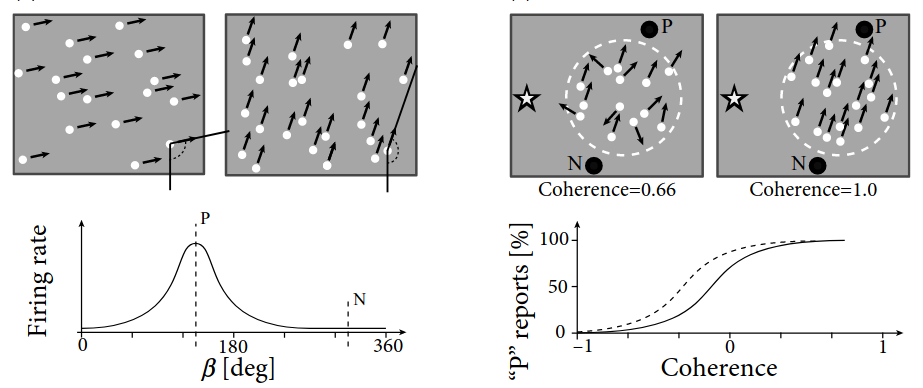
\includegraphics[width=\textwidth]{monkey2.png}
    \caption{Random dot stimuli and perception of motion.}
    \label{monkey2}
    \end{center}
\end{figure}

An electrode in MT can be used not only to record neural activity, but also to stimulate a cluster of neurons in the neighborhood of the electrode. Since neighboring neurons have similar preferred directions of motion, current injection into the electrode can bias the perception of the monkey in favor of the neurons' preferred direction, even if the random dot pattern has no or only a small amount of coherence (\autoref{monkey2}). 

This indicates that \textbf{the perceptual decision of the monkey relies on the motion information represented in the activity of MT neurons (\cite{Salzman 1990} Salzman 1990)}.

\subsection{Place of decision making}

While the monkey's perceptual decision is influenced by the manipulation of MT neurons, this result does not imply that the decision itself is made in MT. It is likely to be made at a later stage, in an area that uses the information of MT neurons.

Unfortunately, to this day, people still do not know the exact location where decisions are made. However, an interesting observation has been made in the lateral intra-parietal (LIP) area during experiments of perceptual decision making with moving random dot stimuli (\cite{Roitman and Shadlen 2002} Roitman and Shadlen 2002). 

Area LIP is located in the visual processing stream between the primary visual cortex and the frontal eye field region involved in control of saccadic eye movements. Neurons in area LIP respond during the preparation of saccadic eye movements. Different neurons in LIP have different receptive fields. The location of the receptive field corresponds to a potential target region of eye movements. In other words, a LIP neuron responds just before a saccadic eye movement into its receptive field occurs.

\begin{figure}[h]
    \begin{center}
    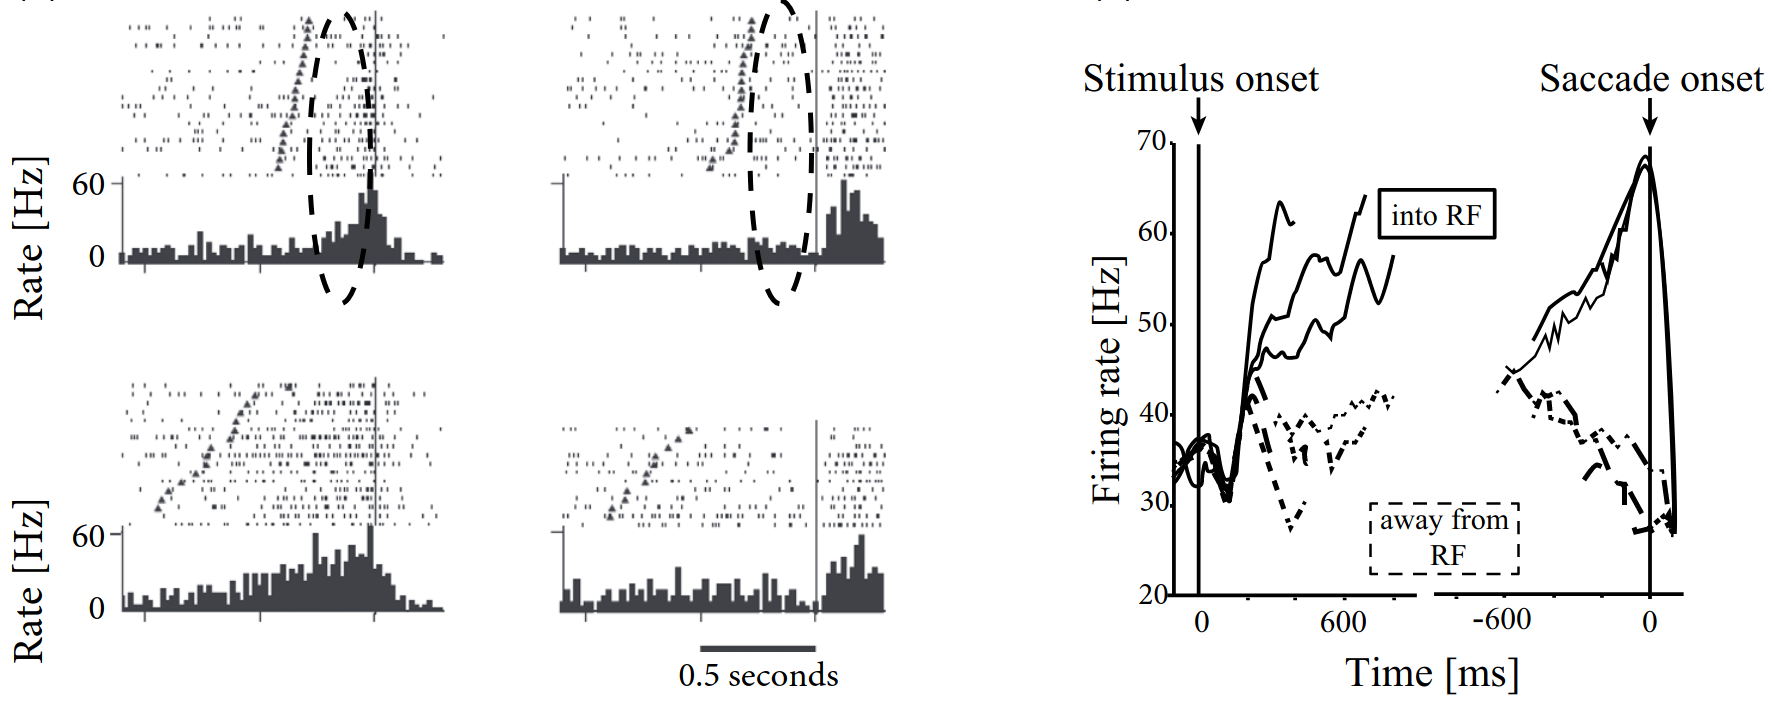
\includegraphics[width=1\textwidth]{LIP.png}
    \caption{Neuronal responses in the LIP area during saccadic eye movements.}
    \label{LIP}
    \end{center}
\end{figure}

As in the previous subsection, monkeys in the experiment by Roitman and Shadlen are trained to indicate the direction of a moving dot pattern by saccadic eye movements to one of two visual targets. The first target is located in the receptive field of a LIP neuron, so the recorded neuron is expected to respond whenever the monkey prepares a movement to this target. The second target is located in the opposite direction. The task is designed such that a random dot stimulus moving toward the first target indicates that the monkey should make an eye movement toward it; the correct response to a stimulus moving in the opposite direction is a saccade to the second target. The difficulty of the task can be varied by changing the fraction of coherently moving dots. The behavioral reaction time of the monkey was measured as a function of stimulus coherence. At the same time, the activity of neurons in LIP was recorded (\autoref{LIP}).

Roitman and Shadlen found that, \textbf{during the presentation of the moving dot stimulus, the activity of LIP neurons increased}. The rate of increase after stimulus onset was higher for stimuli with a large fraction of coherent points than for stimuli with little or no coherence. Importantly, when the responses were averaged and aligned to the onset of the saccade, LIP neurons always reached the same level of activity just before a saccade into their receptive field (\autoref{LIP}).

These findings are consistent with the idea that the decision to perform a saccade occurs at the moment when LIP neurons reach a threshold value. For stimuli with a high degree of coherence, the activity increases more rapidly, the threshold is reached earlier, and reaction times are shorter than for stimuli with a low degree of coherence. Therefore, Roitman and Shadlen suggest that \textbf{``a threshold level of LIP activity appears to mark the completion of the decision process" (\cite{Roitman and Shadlen 2002} Roitman and Shadlen 2002)}.

\section{Competition through common inhibition}

The essential features of the experiments of Roitman and Shadlen (2002) can be described by a simple model of decision making where neuronal populations compete with each other through shared inhibition.

We consider a network of spiking neurons (\autoref{competition}) consisting of \textbf{two excitatory populations interacting with a common pool in inhibitory neurons (\cite{Y. Wang 2002} Y. Wang 2002)}. Within the two excitatory populations neurons are randomly connected with connection weight $w_{EE}$. Connections to and from the inhibitory populations have weights $w_{IE}$ and $w_{EI}$, respectively. Neuronal parameters and connection weights are adjusted such that, in the absence of external input, all neurons exhibit spontaneous activity at low firing rates. In other words, the network is in a state of asynchronous irregular firing.


\begin{figure}[h]
    \begin{center}
    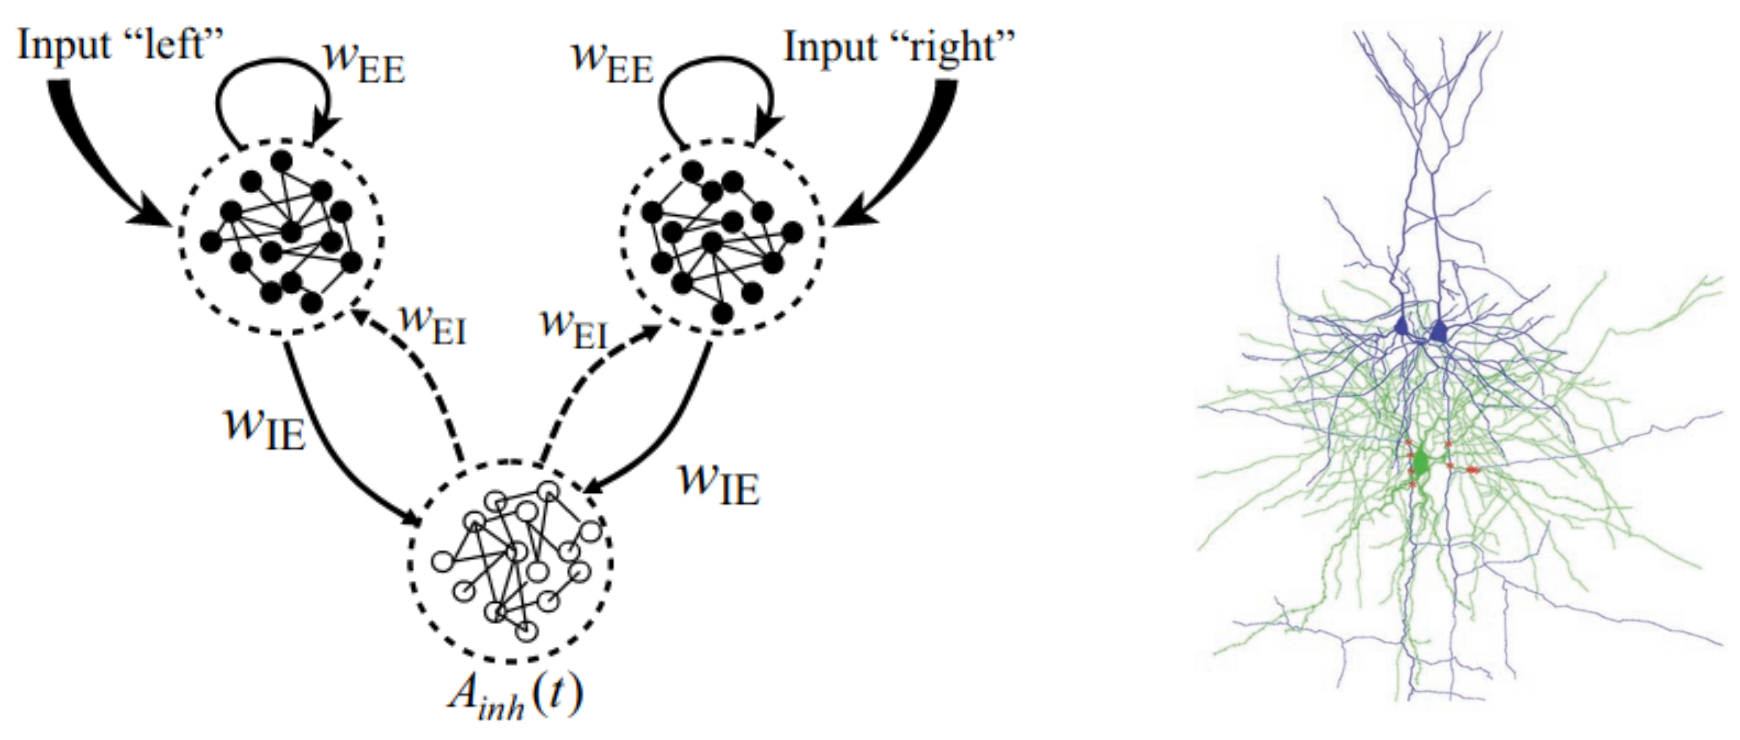
\includegraphics[width=0.9\textwidth]{competition1.png}
    \caption{Competition through common inhibition.}
    \label{competition}
    \end{center}
\end{figure}

\newpage
Stimulation corresponds to a positive mean input into one or both groups of excitatory neurons. For example, for a description of the experiments of Roitman and Shadlen discussed in the previous section, we can identify input into population 1 as indicating coherent motion of the random dot pattern to the left whereas input into population 2 indicates motion to the right (\autoref{competition}). Since the stimulus in the experiments has a random component (e.g., the fraction of coherent dots is less than 100\%), the input into each population is described as a mean plus some noise.

If the pattern has a high degree of coherence and moves to the left, the mean input to population 1 is high. This induces a high activity $A_{E,1}$ which in turn excites the inhibitory population which transmits inhibition to both excitatory pools. However, only the stimulated pool can overcome the inhibition so that the activity of the other excitatory population is suppressed. Since, at most one of the two populations can be active at the same time, the two populations are said to ``compete" with each other. The competition is induced by the shared inhibition. If the external stimulus favors one of the two populations, the population receiving the stronger stimulus ``wins" the competition. In the absence of external stimulation, or for a weak unbiased stimulus, both populations exhibit low activity.

\begin{figure}[h]
    \begin{center}
    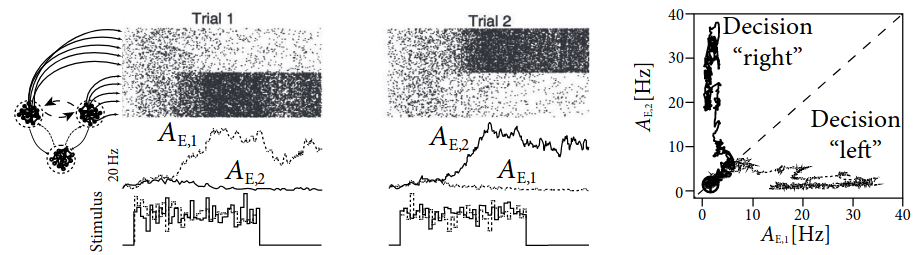
\includegraphics[width=\textwidth]{competition2.png}
    \caption{Dynamics of competition.}
    \label{competition2}
    \end{center}
\end{figure}

To highlight the dynamics of competition, let us now focus on a strong, but unbiased stimulus. Here, unbiased means that, after stimulus onset, both excitatory populations receive an input of the same mean, but with a different realization of the noise (\autoref{competition2}). Immediately after the onset of stimulation, both excitatory populations increase their firing rates. Soon afterward, however, one of the activities grows further at the expense of the other one, which is suppressed. The population which develops a high activity is called the ``winner" of the competition. In the next section, we will show mathematically how the shared inhibition induces a competition between the two excitatory populations.

\section{Dynamics of decision making}

In this section, we present a mathematical analysis of decision making in models of interacting populations. We start in Section 4.1 with the rate equations for a model with three populations, two excitatory ones which interact with a common inhibitory population. In Section 4.2, the rate model with three populations is reduced to a simplified system described by two differential equations. The fixed points of the two-dimensional dynamical system are analyzed in the phase plane in Section 4.3 for several situations relevant to experiments on decision making. Finally, in Section 4.4, the formalism of competition through shared inhibition is generalized to the case of $K$ competing populations.

\subsection{Model with three populations}

To study the behavior of homogeneous populations of neurons, we use the rate model commonly employed in computational neuroscience. Let $A(t)$ represent the average firing rate of a population of homogeneous neurons, and let the input potential be denoted as $h(t)$. Let $F$ be the gain function, then the population activity can be expressed as
$$A(t)=F(h(t)).$$
We use an exponential convolution kernel to represent the decay of the current, then
$$h(t)=\frac{R}{\tau_m}\int_{0}^{\infty}e^{-\frac{s}{\tau_m}}I(t-s)ds,$$
where $\tau_m$ is the membrane time constant and $R$ is the membrane resistance. By applying integration by parts, the above expression is equivalent to the equation
$$\tau_m\frac{dh(t)}{dt}=-h+RI(t),$$
Therefore, \textbf{the general form of the rate model} is
\begin{equation}
    \begin{aligned}
        A(t)&=F(h(t))\\
        \tau_m\frac{dh(t)}{dt}&=-h+RI(t)
    \end{aligned}
\end{equation}\label{general rate model}

In order to analyze the model of \autoref{competition}, we use \autoref{general rate model} and formulate for each of the three interacting populations a differential equation for the input potential. Let $g_E$ and $g_{inh}$ be the gain functions of excitatory and inhibitory neurons respectively. Then \textbf{the competition rate model} is

\begin{equation}
    \begin{aligned}
        A_{E,1}&=g_E (h_{E,1})\\
        A_{E,2}&=g_E (h_{E,2})\\
        A_{inh}&=g_{inh} (h_{inh})\\
        \tau_E \frac{dh_{E,1}}{dt}&=-h_{E,1}+w_{EE}g_E (h_{E,1})+w_{EI}g_{inh} (h_{inh})+RI_1\\
        \tau_E \frac{dh_{E,2}}{dt}&=-h_{E,2}+w_{EE}g_E (h_{E,2})+w_{EI}g_{inh} (h_{inh})+RI_2\\
        \tau_{inh} \frac{dh_{inh}}{dt}&=-h_{inh}+w_{IE}g_E (h_{E,1})+w_{IE}g_{E} (h_{E,2}).
    \end{aligned}
\end{equation}\label{competition rate model}

\noindent
Here $w_{EE}$ denotes the strength of recurrent coupling within each of the excitatory populations and $w_{EI}$ the coupling from the inhibitory to the excitatory population of neurons. Inhibitory neurons are driven by the input from excitatory populations via connections of strength $w_{IE}$. We assume that inhibitory neurons have no self-coupling, but feed their activity $A_{inh}$ back to both excitatory populations with a negative coupling coefficient, $w_{EI} < 0$. Note that the two excitatory populations are completely equivalent, i.e., they contain neurons of the same type and the same coupling strength. However, the two populations receive separate inputs, $I_1$ and $I_2$, respectively. We call an input ``biased" (i.e., favoring one of the two options represented by the excitatory populations) if $I_1 \neq I_2$. We emphasize that the only interaction between the two excitatory populations is indirect via the shared inhibitory population.

\subsection{Effective inhibition}

The system of three differential equations \autoref{competition rate model} is still relatively complicated. We attempt to transform it into a two-dimensional system of equations in order to utilize the powerful mathematical tools of phase plane analysis.

To do so, we make two assumptions. \textbf{First, we assume that the membrane time constant of inhibition is shorter than that of excitation, $\mathbf{\tau_{inh} \ll \tau_{E}}$.} Formally, we consider the limit of a separation of time scales $\tau_{inh} / \tau_{E} \to 0$. Therefore we can treat the dynamics of $h_{inh}$ in \autoref{competition rate model} as instantaneous, so that the inhibitory potential is always at its fixed point
$$h_{inh}=w_{IE}[g_E (h_{E,1})+g_E (h_{E,2})].$$
Actually, inhibitory neurons do indeed fire at higher firing rates than excitatory ones and are in this sense ``faster". However, this observation on its own does not imply that the membrane time constants of excitatory and inhibitory neurons, respectively, would differ by a factor of 10 or more; in fact, they don’t. Nevertheless, a focus on the raw membrane time constant is also too limited in scope, since we should also take into account synaptic processes. Excitatory synapses typically have an NMDA component with time constants in the range of a hundred milliseconds or more, whereas inhibitory synapses are fast.

Intuitively, the assumption of a separation of time scales implies that inhibition reacts faster to a change in the input than excitation. In the following we simply assume the separation of time scales between inhibition and excitation, because it enables a significant simplification of the mathematical treatment. Essentially, it means that the variable $h_{inh}$ can be removed from the system of three equations
\begin{equation}
    \begin{aligned}
        \tau_E \frac{dh_{E,1}}{dt}&=-h_{E,1}+w_{EE}g_E (h_{E,1})+w_{EI}g_{inh} (w_{IE}[g_E (h_{E,1})+g_E (h_{E,2})])+RI_1\\
        \tau_E \frac{dh_{E,2}}{dt}&=-h_{E,2}+w_{EE}g_E (h_{E,2})+w_{EI}g_{inh} (w_{IE}[g_E (h_{E,1})+g_E (h_{E,2})])+RI_2.
    \end{aligned}
\end{equation}\label{reduction1}

The second assumption is not absolutely necessary, but it makes the remaining two equations more transparent. \textbf{The assumption concerns the shape of the gain function of inhibitory neurons. We require a linear gain function} and set
$$g_{inh}(h_{inh})=\gamma h_{inh}$$
with a slope factor $\gamma > 0$. Set parameter $\alpha=-\gamma w_{EI}w_{IE}>0$. Then \autoref{reduction1} becomes
\begin{equation}
    \begin{aligned}
        \tau_E \frac{dh_{E,1}}{dt}&=-h_{E,1}+(w_{EE}-\alpha)g_E (h_{E,1})-\alpha g_E (h_{E,2})+RI_1\\
        \tau_E \frac{dh_{E,2}}{dt}&=-h_{E,2}+(w_{EE}-\alpha)g_E (h_{E,2})-\alpha g_E (h_{E,1})+RI_2
    \end{aligned}
\end{equation}\label{reduction2}

\noindent
Thus, the model of three populations has been replaced by a model with two excitatory populations that interact with an effective inhibitory coupling of strength $\alpha$. (\autoref{reduction-pic})

\begin{figure}[h]
    \begin{center}
    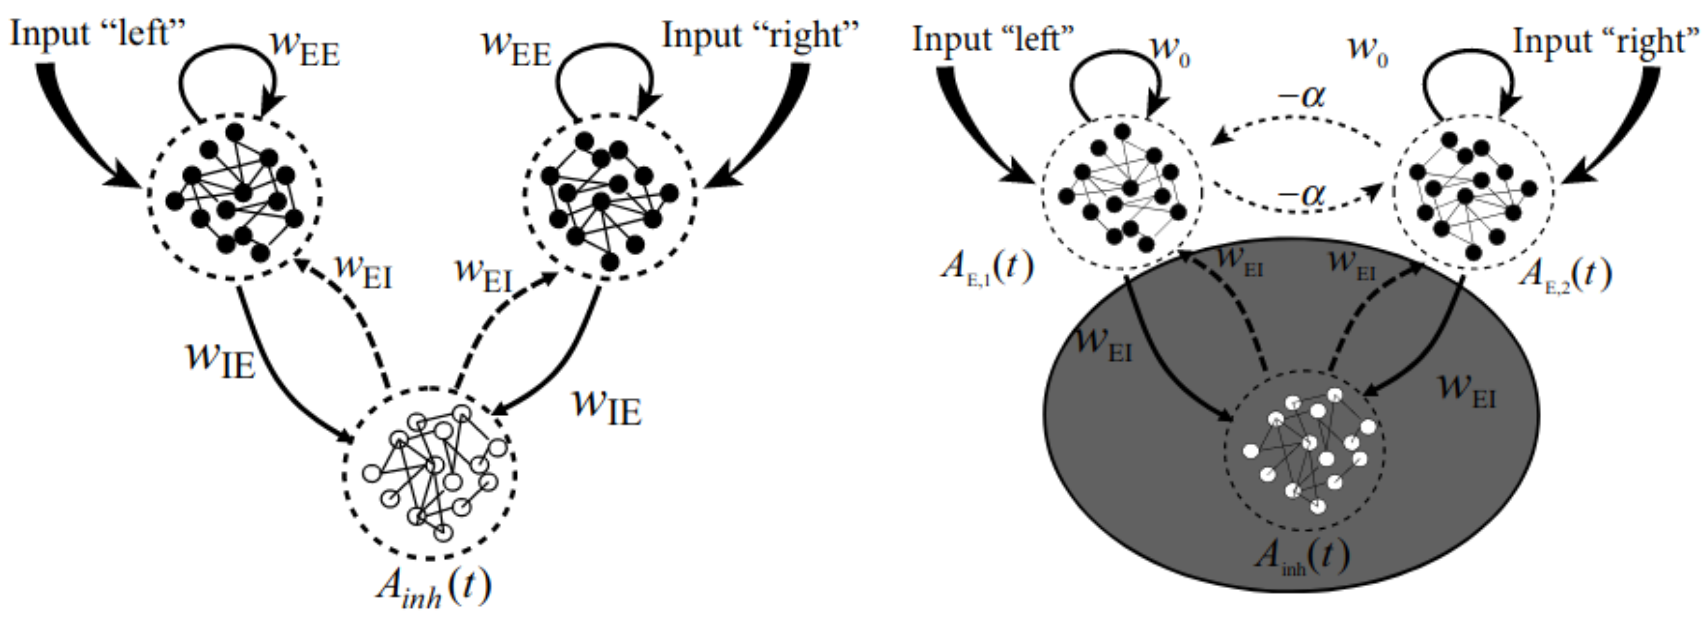
\includegraphics[width=\textwidth]{competition-pic.png}
    \caption{The equivalent inhibitory connections after dimensionality reduction.}
    \label{reduction-pic}
    \end{center}
\end{figure}

Even though neurons make either excitatory or inhibitory synapses, the above derivation shows that, under appropriate assumptions, there is a mathematically equivalent description where explicit inhibition by inhibitory neurons is replaced by effective inhibition between excitatory neurons. The effective inhibitory coupling allows us to discuss competition between neuronal groups in a transparent manner.

\subsection{Phase plane analysis}

\textbf{(1)} $\mathbf{I_1=I_2=0}:$ In the left image of \autoref{phase-analysis}, the nullclines $dh_{E,1}/dt = 0$ and $dh_{E,2}/dt = 0$ are shown as a function of $h_{E,1}$ (horizontal axis) and $h_{E,2}$ (vertical axis). There is a single crossing point corresponding to a stable fixed point close to $h_{E,1} = h_{E,2} = 0$. Arrows indicate the flow toward the fixed point.

\textbf{(2)} $\mathbf{I_1 > 0 = I_2}:$ In the middle image of \autoref{phase-analysis}, if a stimulus $I_1 > 0$ favors the first population, the fixed point moves to an asymmetric position where population 1 exhibits much stronger activity $A_{E,1} = g(h_{E,1})$ than population 2. Note that, at the fixed point, $h_{E,2}\gg 0$. In other words, the effective interaction between the two populations causes a strong inhibitory input potential to population 2. This is a characteristic feature of a competitive network. If one of the populations exhibits a strong activity, it inhibits activity of the others so that only the activity of a single winning population ``survives". 

\textbf{(3)} $\mathbf{I_1=I_2>0}:$ In the right image of \autoref{phase-analysis}, a particularly interesting situation arises with a strong but unbiased stimulus. with a strong unbiased stimulus $I_1 = I_2 \gg 0$, three fixed points exist. The symmetric fixed point $h_{E,1} = h_{E,2}$ is a saddle point and therefore unstable. The two other fixed points occur at equivalent positions symmetrically to the left and right of the diagonal. These are the fixed points that enforce a decision ``left" or ``right". It depends on the initial conditions, or on tiny fluctuations in the noise of the input, whether the system ends up in the left or right fixed point. 

\begin{figure}[h]
    \begin{center}
    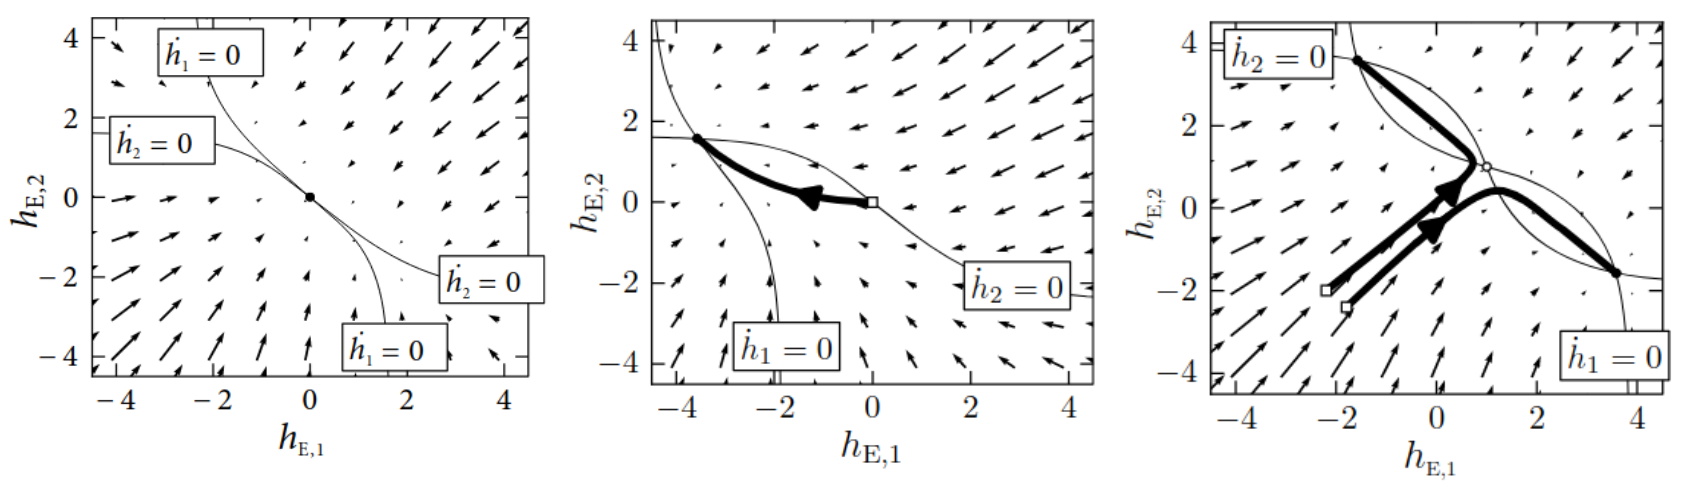
\includegraphics[width=\textwidth]{phase-analysis.png}
    \caption{Phase plane analysis of the competition model.}
    \label{phase-analysis}
    \end{center}
\end{figure}

\textbf{The phase plane analysis of the two-dimensional system correctly reflects the dynamics observed in the simulations of the model with populations of hundreds of spiking neurons in \autoref{competition2}.}

\subsection{Formal winner-take-all networks}

The arguments that were developed above for the case of a binary choice between two options can be generalized to a situation with $K$ possible outcomes. Each outcome is represented by one population of excitatory neurons. Analogous to the arguments in \autoref{reduction-pic}, we work with an effective inhibition of strength $\alpha > 0$ between the $K$ pools of neurons and with a self-interaction of strength $w_0$ within each pool of neurons.

The activity of population $k$ is then
$$A_k(t)=g(h_k(t))$$
with input potential
$$\tau \frac{dh_k(t)}{dt}=-h_k(t)+w_0g(h_k(t))-\alpha\sum_{j\neq k}w_{kj}g(h_j(t))+RI_k$$
where the sum runs over all neurons $1 \leq j \leq K$, except neuron $k$. Note that we assume here a network of interacting populations, but it is common to draw the network as an interaction between formal units. Despite the fact that, in our interpretation, each unit represents a whole population, the units are often called ``artificial neurons" (\autoref{winner}). Winner-take-all networks are a standard topic of artificial neural networks (\cite{Hertz 1991} Hertz 1991; \cite{Kohonen 1984} Kohonen 1984; \cite{Haykin 1994} Haykin 1994). 


\begin{figure}[h]
    \begin{center}
    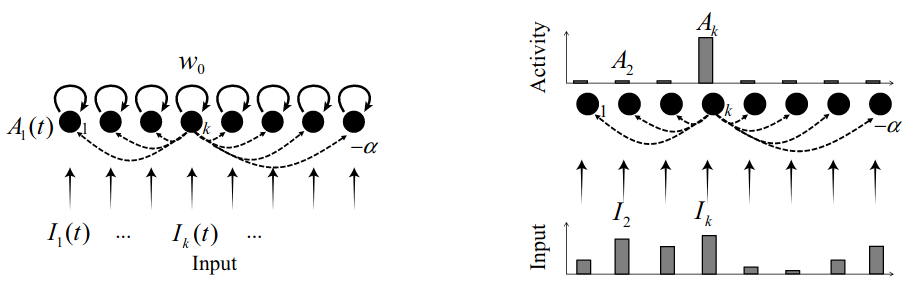
\includegraphics[width=0.9\textwidth]{winner.png}
    \caption{Formal winner-take-all network.}
    \label{winner}
    \end{center}
\end{figure}

Consider a network of formal neurons described by activities $A_k = [1 + tanh(h - \theta)] A_{max}/2$. We work in unit-free variables and set $A_{max} = 1$ and $\theta = 5$. Thus, for an input potential $h = 0$ the activity is nearly zero while for $h = 10$ it is close to 1. The input potential contains contributions from external input as well as contributions from recurrent interactions within the network. Suppose that for all times $t < t_0$ the external input vanishes, $I_k = 0$ for all $k$. Thus, at time $t_0$ the input potential $h_k$ and the activity $A_k$ are negligible for all units $k$. Therefore the interactions within the network are negligible as well.

At time $t_0$ the input is switched on to a new fixed value $I_k$ which is different for each neuron (\autoref{winner}). The activity of the neuron $k$ which receives the strongest input grows more rapidly than that of the others so that its activity also increases more rapidly. The strong activity of neuron $k$ inhibits the development of activity in the other neurons so that, in the end, the neuron with the strongest input wins the competition and its activity is the only one to survive.

\section{Alternative decision models}

In the previous two sections, we discussed decision models as the competitive interaction between two or more populations of excitatory neurons. In this section we present two different models of decision making, i.e., the energy picture in Section 5.1 and the drift diffusion model in Section 5.2. Both models are phenomenological concepts to describe decision making. However, both models are also related to the phase diagram of the model of two neuronal populations, encountered in Section 4.

\subsection{The energy picture}

Binary decisions can be visualized as a ball in a hilly energy landscape. Once the ball rolls in a certain direction, a decision starts to form. The decision is finalized when the ball approaches the energy minimum (\autoref{ball}). The decision variable $x$ reflects a decision for option A if it approaches a fixed point in the neighborhood of $x \thickapprox  1$, and a decision for option B for $x \thickapprox  -1$. If the variable $x$ is trapped in a minimum close to $x = 0$, no decision is taken.

\begin{figure}[h]
    \begin{center}
    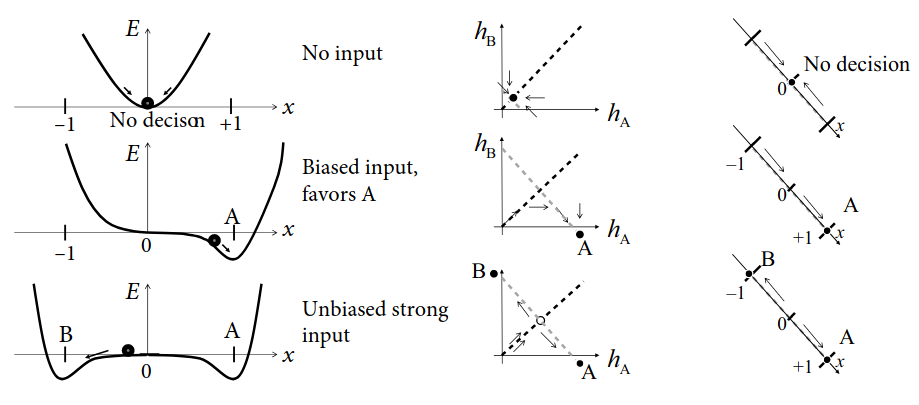
\includegraphics[width=\textwidth]{competition4.png}
    \caption{The energy picture of decision making.}
    \label{ball}
    \end{center}
\end{figure}

The dynamics of the decision process can be formulated as gradient descent
$$\frac{dx}{dt}=-\eta \frac{dE}{dx}$$
with a positive constant $\eta$. In other words, in a short time step $\Delta   t$, the decision variable moves by an amount $-\eta \Delta t dE/dx$. Thus, if the slope is positive, the movement is toward the left. As a result, the movement is always downhill, so that the energy decreases along the trajectory $x(t)$. We can calculate the change of the energy along the trajectory:
$$\frac{dE(x(t))}{dt}=\frac{dE}{dx}\frac{dx}{dt}=-\eta \left( \frac{dE}{dx}\right)^2\leq 0$$
Therefore the energy plays the role of a Liapunov function of the system, i.e., a quantity that cannot increase along the trajectory of a dynamical system.

Interestingly, the energy picture can be related to the phase plane analysis of the two dimensional model that we encountered earlier in \autoref{phase-analysis}. The diagonal of the phase plane plays the role of the boundary between the options A and B while the variable $x$ indicates the projection onto an axis orthogonal to the diagonal. Position $x = 0$ is the unbiased, undecided position on the diagonal. In the case of strong unbiased input, the one-dimensional flow diagram of the variable $x$ presents a reasonable summary of the flow pattern in the two-dimensional system, because the saddle point in the phase plane is attractive along the diagonal and is reached rapidly while the flow in the perpendicular direction is much slower (\cite{X. Wang 2002} X. Wang 2002; \cite{Bogacz 2006} Bogacz 2006; \cite{Wong and X. Wang 2006} Wong and X. Wang 2006).

The above arguments regarding the Liapunov function of the network can be made more precise and formulated as a general theorem (\cite{Cohen and Grossberg 1983} Cohen and Grossberg 1983; \cite{Hopfield 1984} Hopfield 1984). We consider an arbitrary network of $K$ neuronal populations $1 \leq j \leq K$ with population rate $A_j = g(h_j) \geq 0$ where $g$ is a gain function with derivative $g' > 0$ and $h$ follows the dynamics
$$\tau\frac{dh_j}{dt}=-h_j+RI_j+\sum\limits_k w_{jk}g(h_k)$$
with fixed inputs $I_j$. If the coupling is symmetric, i.e., $w_{ij} = w_{ji}$, then the energy
$$E=-\sum\limits_i\sum\limits_j w_{ij} A_i A_j-\sum\limits_i A_i RI_i+\sum\limits_i\int_{0}^{A_i}g^{-1}(a)da$$
is \textbf{a Liapunov function of the dynamics}. The proof follows by taking the derivative. We exploit the fact that $w_{ij} = w_{ji}$ and apply the chain rule $dA_i/dt = g'(h_i)dh_i/dt$, then 
\begin{equation*}
    \begin{aligned}
        \frac{dE}{dt}&=-\sum\limits_i \left[\sum\limits_j w_{ij}A_j\right]g'(h_i)\frac{dh_i}{dt}-\sum\limits_i RI_ig'(h_i)\frac{dh_i}{dt}+\sum\limits_i g^{-1}(A_i)g'(h_i)\frac{dh_i}{dt}\\
        &=-\tau \sum\limits_i g'(h_i)\left[\frac{dh_i}{dt}\right]^2 \leq 0 \\
    \end{aligned}
\end{equation*}
Since the neuronal gain function stays below a biologically sustainable firing rate $g(x) \leq A_{max}$, the energy is bounded from below. Therefore the flow of a symmetric network of interacting populations will always converge to one of the stable fixed points corresponding to an energy minimum, unless the initial condition is chosen to lie on an unstable fixed point, in which case the dynamics stays there until it is perturbed by some input.

\subsection{Drift-diffusion model}

The drift-diffusion model is a phenomenological model to describe choice preferences and distributions of reaction times in binary decision making tasks (\cite{Ratcliff and Rouder 1998} Ratcliff and Rouder 1998). At each trial of a decision experiment, a decision variable $x$ is initialized at time $t_0$ at a value $x(t_0) = x_0$. Thereafter, the decision variable evolves according to
$$\frac{dx}{dt}=(I_A-I_b)+\sigma \xi (t)$$
where $\xi (t)$ is Gaussian white noise of unit mean and variance $\sigma^2$. An input $I_A > I_B$ causes a ``drift" of the variable $x$ toward positive values while the noise $\xi$ leads to a ``diffusion"-like motion of the trajectory, hence the name ``drift-diffusion model".

\begin{figure}[h]
    \begin{center}
    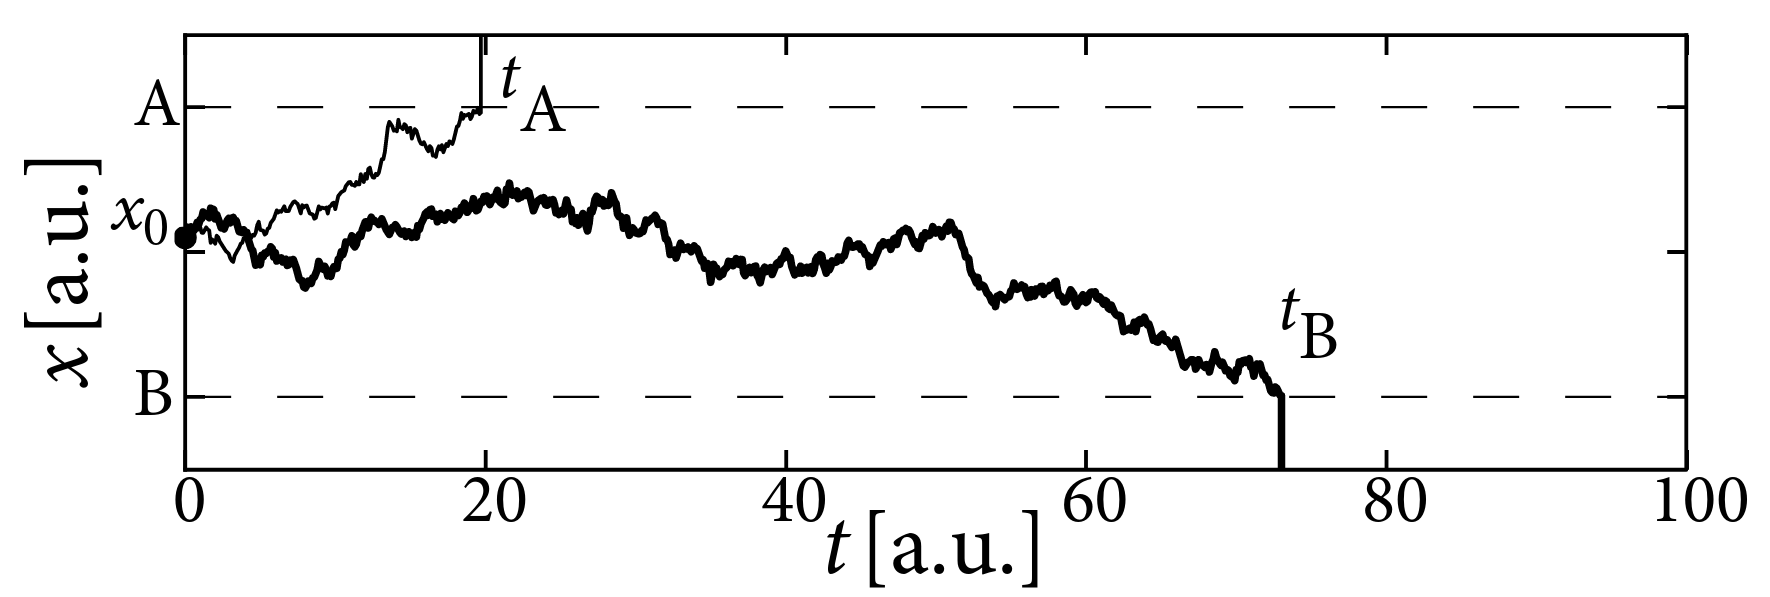
\includegraphics[width=0.7\textwidth]{diffusion.png}
    \caption{The drift-diffusion model.}
    \label{diffusion}
    \end{center}
\end{figure}

The reaction time is the time at which the variable $x$ reaches one of two thresholds, $\theta_A$ or $\theta_B$, respectively (\autoref{diffusion}). For example $t_B$, defined by $t_B = min \{t|x(t) = \theta_B\}$, is the reaction time in a trial where the choice falls on option $B$. Parameters of the phenomenological drift-diffusion model are the values of thresholds $\theta_A$ and $\theta_B$, and the strength of the input $I_A-I_B$ compared to that of the noise. The initial condition $x_0$ can be identical in all trials or chosen in each trial independently from a small interval that reflects uncontrolled variations in the bias of the subject. The time $t_0$ is typically the moment when the subject receives the choice stimulus, but it is also possible to start the drift-diffusion process a few milliseconds later so as to account for the propagation delay from the sensors to the brain (\cite{Ratcliff and Rouder 1998} Ratcliff and Rouder 1998; \cite{Ratcliff and McKoon 2008} Ratcliff and McKoon 2008).

\section{Human decisions, determinism and free will}

In the previous section, we compared the process of decision making to a ball in an energy landscape. However, as outlined in the introduction to this report, decision making incorporates a broad set of phenomena and processes (\cite{Rangel 2008} Rangel 2008; \cite{Sanfey and Chang 2008} Sanfey and Chang 2008). Here we sketch a link from the simplified model from decision making to the bigger picture.

Voluntary control of actions can be understood in opposition to pure reflexes. The movement of our arms and legs is controlled by muscles which in turn receive action potentials from the brain via the spinal cord. The human cortex contains several areas that are involved in voluntary actions. The question of where and how the brain controls our decisions and represents our will has triggered the research field of ``neuroscience of volition"  (\cite{Haggard 2008} Haggard 2008).

\subsection{The Libet experiment}

The classic experiment in the research field of human volition was performed by Libet (1985). In this experiment, subjects decide on their own when to move their right hand. After each trial, subjects report when they felt the ``urge to move", with respect to a rapidly rotating hand of a clock. The reported ``urge to move" is in fact about 200 ms earlier than the actual movement. Most interestingly, however, electrical brain activity measured by EEG recordings indicates that the brain exhibits signals of preparatory activity several hundred milliseconds before the reported ``urge to move". Thus, if we agree to interpret the felt ``urge to move" as the conscious decision to move the hand, then we must also accept the fact that the brain has unconsciously prepared our decision.

A modern and debated variant of the Libet experiment is shown in \autoref{game1}. The main difference to the original Libet experiment (where the decision was limited to ``move" or ``not move") is that subjects now hold two buttons, one in the left and the other in the right hand (\cite{Soon 2008}Soon 2008). Subjects are free to decide when to move and press either of the two buttons. While subjects perform the experiment, they watch a stream of letters at a rate of two letters per second. At the end of each trial, they indicate at which letter they had felt the ``urge to move". The reported letter serves as a timing reference for the subsequent analysis.

During the experiment, brain activity was recorded through functional magnetic resonance imaging (FMRI). Using statistical pattern classification techniques, the authors aimed at predicting the final response outcome (left or right) based on the activity patterns in localized brain areas. If brain activity contained no cue about the final decision, the prediction would always be 50\%. However, the authors found that activity patterns in fronto-polar cortex 5 seconds before the reported ``urge to move" allowed them to predict the final choice (left or right) with a precision of 55-60\% (\cite{Soon 2008} Soon 2008), which is above chance but far from a reliable prediction.

\begin{figure}[h]  
    \centering  
    \begin{minipage}{0.45\textwidth} 
        \centering  
        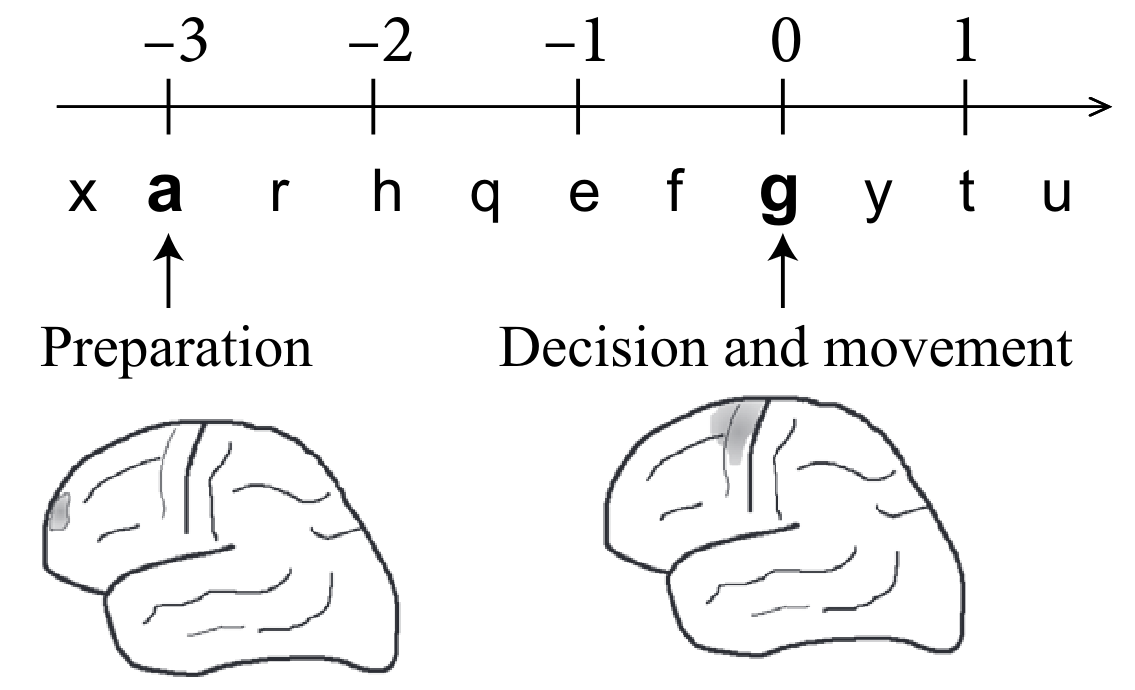
\includegraphics[width=\textwidth]{game1.png} 
        \caption{The Libet experiment.}
        \label{game1}  
    \end{minipage}  
    \hspace{0.1\textwidth}
    \begin{minipage}{0.3\textwidth} 
        \centering  
        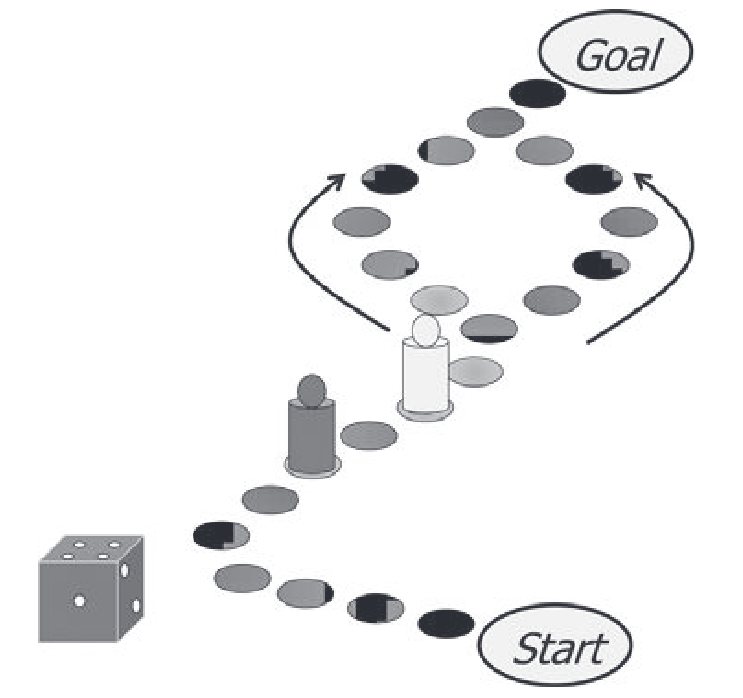
\includegraphics[width=\textwidth]{game2.png} 
        \caption{Board Game.}
        \label{game2}  
    \end{minipage}  
\end{figure} 

\subsection{Relevant and irrelevant decisions - a critique}

In a naive interpretation, the results seem to suggest that the brain has taken its own decision a long time before the subject becomes aware of it. As Wolfgang Prinz puts it: ``We don't do what we want, but we want what we do" (\cite{Prinz 2004} Prinz 2004). There is little doubt that our actions, plans, and wishes are represented in the brain. Our childhood memories are stored in our brain; our knowledge of the world is memorized in the brain; our values and priorities acquired through education, reading, understanding, trial and error, or simply through being embedded in our culture, must also be stored in the brain. Thus, a large fraction, if not all, of what we consider our conscious personality is located in the brain.

Most actions where we care about our decision are relevant choices. The decision of whether to take the risky shortcut across a busy street or the safer underground pathway depends on what we have experienced in the past. Similarly, the decision in the board game of \autoref{game2} depends on the player's attitude toward risk, which has been formed by previous experiences in similar situations. However, the decision task in the scientific experiment of Libet (1985) or Soon (2008) is a completely irrelevant one. Subjects don't really care whether they move the left or right finger. The decision has nothing to do with life-long experience or attitude toward risk. In cases like this one, any decision is arbitrary and therefore easily influenced by noise. 

Interestingly, even in the irrelevant situation of the experiment of Soon (2008), the predictive power of the brain activity five seconds before the conscious ``urge to move" is only in the range of 60\%. Moreover, in a different experimental design, the subject could ``veto" at the last moment a previously prepared movement suggesting the possibility of voluntary inhibition of actions that are only weakly predicted (\cite{Brass and Haggard 2007} Brass and Haggard 2007). Finally, there is also the problem of whether we can really identify a reported ``urge to move" with a precise moment of decision. If we take the picture of the ball in the energy landscape, the ball starts to roll in a certain direction while still remaining in the flat region. But this does not yet imply a final decision, because novel input could tilt the energy landscape in the opposite direction.


\section{Summary}

Decisions are prepared and made in the brain so that numerous physiological correlates of decision making can be found in the human and monkey cortex. The fields of cognitive neuroscience associated with these questions are called ``neuroeconomics" and ``neuroscience of volition".

An influential computational model describes decision making as the competition of several populations of excitatory neurons which share a common pool of inhibitory neurons. Under suitable conditions, the explicit model of inhibitory neurons can be replaced by an effective inhibitory coupling between excitatory populations. In a rate model, the competitive interactions between two excitatory populations can be understood using phase plane analysis. Equivalently, the decision process can be described as downward motion in an energy landscape which plays the role of a Liapunov function. The energy picture is valid for any rate model where all units of the network are coupled by symmetric interactions.

The drift-diffusion model, which has been used in the past as a black-box model for reaction time distributions and choice preferences, can, under appropriate assumptions, be related to a rate model of competitively interacting populations of neurons.

%%----------- 参考文献 -------------------%%
%在reference.bib文件中填写参考文献,此处自动生成
\newpage
\reference




%------------------------附录------------------------%

































\end{document}